\begin{appendices} \label{APPENDIX}
\section{The Type 1 Diabetes ODE and Data} \label{general_appendix}
\subsection{The ODE System, States, and Parameters}
Below is the full set of 12 states in the T1D ODE model, along with their corresponding ODEs. We also present a table containing all parameter values and their biological significance. \\
\\
Definitions and units for each state are presented in Table \ref{table:StateNotationAppendix}.

\begin{table}[H]
\centering
        \begin{tabular}{c|c|c|c|c}
        \cline{1-5}
            \textbf{State}  & \textbf{Units} &  \textbf{Meaning} & \textbf{Initial Value} & \textbf{Corresponding Equation}\\
            \hline
            B & mg & Healthy $\beta$-cell Population & 300 mg & \ref{eq:dB/dt}\\
            G & mg/dl & Glucose Level & 100 mg/dl & \ref{eq:dG/dt}\\
            I & $\mu$ U & Insulin Level & 10 $\mu$ U & \ref{eq:dI/dt}\\
            M & cells/ml & Macrophage Population & 4.77e05 cells/ml & \ref{eq:dM/dt}\\
            $M_a$ & cells/ml & Active Macrophage Population & 0 cells/ml & \ref{eq:dM_a/dt}\\
            $B_a$ & cells/ml & Apoptotic $\beta$-cell Population & 0 cells/ml & \ref{eq:dB_a/dt}\\
            $B_n$ & cells/ml & Necrotic $\beta$-cell Population & 0 cells/ml & \ref{dB_n/dt}\\
            D & cells/ml & Immunogenic DC Population & 0 cells/ml & \ref{eq:dD/dt}\\
            tD & cells/ml & Tolerogenic DC Population & 0 cells/ml & \ref{eq:tD/dt}\\
            E & cells/ml & Effector T-cell Population & 0 cells/ml & \ref{eq:dE/dt}\\
            R & cells/ml & Regulatory T-cell Population & 0 cells/ml & \ref{eq:dR/dt}\\
            Em & cells/ml & Memory T-cell Population & 0 cells/ml & \ref{dE_m/dt}
        \end{tabular}
    \caption{State variables in the T1D model and their associated units, biological meaning, and initial value. Table is taken from \cite{WuThesis}}
    \label{table:StateNotationAppendix} 
\end{table}




\begin{equation}\label{eq:dM/dt}
    \frac{d}{dt}M = J+(k+b)M_{a}-cM-f_{M}MB_{a}-f{M}MB_{n}-e_{1}M(M+M_{a}),
\end{equation}\\

\begin{equation}\label{eq:dM_a/dt}
    \frac{d}{dt}M_{a} = f_{M}MB_{a}+f_{M}MB_{n}-kM_a-e_{2}M_{a}(M+M_{a}),
\end{equation}
\begin{equation}\label{eq:dB/dt}
    \frac{d}{dt}B = \alpha_{B}K_{1}(G)B-\delta_{B}B-\eta_{e}(t)K_{2}(E,R)B-W(B,t),
\end{equation}
\begin{equation} \label{eq:dB_a/dt}
    \frac{d}{dt}B_a = \tilde{\delta_B}B+\tilde{\eta_e}K_2(E,R)B+\tilde{W}(B,t)-dB_a-f_{M_a}M_{a}B_a-f_{M_a}M_{a}B_a-f_{tD}(D_{ss}-D)B_a-f_{D}DB_a,
\end{equation}
\begin{equation}\label{dB_n/dt}
    \frac{d}{dt}B_n = dB_a-f_{M}MB_n-f_{M_a}M_{a}B_n-f_{tD}(D_{ss}-D)B_n-f_{D}DB_n,
\end{equation}
\begin{equation}\label{eq:dG/dt}
    \frac{d}{dt}G = R_0-(G_0+S_{I}I)G,
\end{equation}
\begin{equation}\label{eq:dI/dt}
    \frac{d}{dt}I = \sigma_{I}K_{1}(G,G_{I})B-\delta_{I}I,
\end{equation}
\begin{equation}\label{eq:dD/dt}
    \frac{d}{dt}D = f_{tD}B_{n}(D_{ss}-D-tD)+f_{tD}B_{n}tD-b_{DE}ED-\mu_{D}D,
\end{equation}
\begin{equation}\label{eq:tD/dt}
    \frac{d}{dt}tD = f_{tD}B_{a}(D_{ss}-D-tDD)-f_{tD}B_{n}tD-b_{IR}RtD-\mu_{D}tD,
\end{equation}
\begin{equation}\label{eq:dE/dt}
    \frac{d}{dt}E = a_{E}(T_{naive}-E)+b_{P}\frac{DE}{\theta_{D}+D}-r_{am}E+b_{E}DE_{m}-\mu_{E}ER,
\end{equation}
\begin{equation}\label{eq:dR/dt}
    \frac{d}{dt}R= a_R(T_{naive}-R)+b_{p}\frac{tDR}{\theta_D+tD}-r_{am}R+b_{R}tDE_m,
\end{equation}
\begin{equation}\label{dE_m/dt}
    \frac{d}{dt}E_m = r_{am}(E+R)-(a_{Em}+b_ED+b_{R}tD)E_m.
\end{equation}

\vspace{3mm}
Table \ref{table:ParameterNotationAppendix} shows the 53 parameters of the T1D ODE model with their respective units and a brief description.
\subsection{T1D Parameters}
\begin{table}[H] 
\centering
        \hspace*{-2.0cm}\begin{tabular}{c|c|c}
        \cline{1-3}
            \textbf{Parameter}  & \textbf{Units} &\textbf{Description}\\
            \hline
            J & cells ml$^{-1}$ day$^{-1}$ & Resting macrophage influx\\
            k & 1/day & Macrophage deactivation rate\\
            b & 1/day & Recruitment rate of macrophages by activated macrophages\\
            c & 1/day & Macrophage egress rate\\
            $e_1$ & cells$^{-1}$ day$^{-1}$ & Effect of crowding on macrophages\\
            $e_2$ & cells$^{-1}$ day$^{-1}$ & Effect of crowding on active macrophages\\
            $f_M$ & ml cells$^{-1}$ day$^{-1}$ & Rate macrophages engulf necrotic and apoptotic $\beta$-cells\\
            $f_{M_a}$ & ml cells$^{-1}$ day$^{-1}$ & Rate activated macrophages engulf necrotic and apoptotic $\beta$-cells\\
            $\alpha_B$ & ml cells$^{-1}$ day$^{-1}$ & Rate $\beta$-cells are produced from glucose\\
            $G_{hb}$ & mg/dl & Glucose level of half-max $\beta$-cell production\\
            $\delta_B$ & 1/day & $\beta$-cell death rate\\
            $Q_{panc}$ & ml & Volume of mouse pancreas\\
            $B_{conv}$ & cells/mg & $\beta$-cells per milligram\\
            $\eta$ & 1/day & Rate at which T cells eliminate $\beta$-cells\\
            $s_E$ & ml/cells & Relative impact of effector T cells on $\beta$-cell death\\
            $s_R$ & ml/cells & Relative impact of regulatory T cells on $\beta$-cell death\\
            $\alpha_e$ & 1/day & Rate of effector T cell avidity for $\beta$-cells\\
            $\beta_e$ & day & Half-max value for T cell killing of $\beta$-cells\\
            $d$ & 1/day & $\beta$-cell rate of necrosis\\
            $f_D$ & ml cells$^{-1}$ day$^{-1}$ & Rate DCs engulf $\beta$-cells\\
            $f_{tD}$ & ml cells$^{-1}$ day$^{-1}$ & Rate naive or tolerogenic DCs engulf $\beta$-cells\\
            $D_{ss}$ & cells/ml & Steady-state DC population\\
            $R_0$ & mg/dl & Basal rate of glucose production\\
            $G_0$ & 1/day & Rate of glucose decay\\
            $S_I$ & ml $\mu$ U$^{-1}$ day$^{-1}$ & Rate of glucose elimination via insulin\\
            $G_I$ & mg/dl & Glucose level of half-max insulin production\\
            $\sigma_I$ & $\mu$U ml$^{-1}$ day$^{-1}$ mg$^{-1}$& Maximum rate of insulin production by $\beta$-cells\\
            $\delta_I$ & 1/day & Rate of insulin decay\\
            $b_{DE}$ & ml cells$^{-1}$ day$^{-1}$ & Rate of elimination of DCs by effector T cells\\
            $b_{IR}$ & ml cells$^{-1}$ day$^{-1}$ & Rate of elimination of tDCs by regulatory T cells\\
            $\mu_D$ & 1/day & Rate of removal from pancreas for DC and tDC\\
            $a_E$ & 1/day & Rate of initial expansion of naive T cells into effector T cells\\
            $a_R$ & 1/day & Rate of initial expression of naive T cells into regulatory T cells\\
            \multirow{3}{*}{$T_{naive}$} & \multirow{3}{*}{cells/ml} &  \\
            & & Density of naive T cells contributing to initial production of effector and regulatory\\
            & & T cells in the spleen\\
            $b_P$ & 1/day & Maximal expansion rate of effector and regulatory T cells due to DCs\\
            $r_{am}$ & 1/day & Reversion rate of effector and regulatory T cells to memory T cells\\
            $b_E$ & ml day cells$^{-1}$ & Activation rate for effector T cells from memory T cells\\
            $\mu_E$ & 1/day & Rate of effector T cell removal due to regulatory T\\
            $\theta_D$ & 1/day & DC value for half-maximal effector T cell expansion\\
            $b_R$ & ml day cells$^{-1}$  & Activation rate for regulatory T cells from memory T cells\\
            $\mu_R$ & 1/day & Rate of regulatory T cell removal due to effector T\\
            $a_{E_m}$ & 1/day & Death rate of memory T cells\\
            
            
        \end{tabular}
    \caption{Parameters of the T1D model, their associated units, biological meaning, and initial value. Table is taken from \cite{shtylla2019mathematical}.}
    \label{table:ParameterNotationAppendix} 
\end{table}

The data used throughout work with the T1D model comes from \cite{Lietal2009}. Below, find tables for the raw glucose data for each mouse:

\begin{table}[H]
\centering
  \begin{center} 
    \begin{tabular} {c|c|c|c|c|c|c|c|c|c|c}% <-- Alignments: 1st column left, 2nd middle and 3rd right, with vertical lines in between
    \cline{1-11}
      \textbf{Time (weeks)} & 21.061 & 23.08 & 25.012 & 27.025 & 28.992 & 31.023 & 33.092 & 35.025 & 37.059 & 38.995 \\
      \hline
      \textbf{Glucose (mg/dl)} & 186.51 & 224.91 & 259.78 & 183.38 & 205.71 & 235.1 & 220.99 & 249.2 & 253.2 & 266.83\\
      \hline
    \end{tabular}
    \caption{Raw glucose data for \textbf{Mouse 1} from \cite{Lietal2009}.}
    \label{table:Li_Mouse1}
  \end{center}
\end{table}

\begin{table}[H]
\centering
  \begin{center} 
    \begin{tabular} {c|c|c|c|c|c|c|c}% <-- Alignments: 1st column left, 2nd middle and 3rd right, with vertical lines in between
    \cline{1-8}
      \textbf{Time (weeks)} & 21.15 & 25.02 & 27.104 & 31.019 & 33.013 & 35.004 & 36.932\\
      \hline
      \textbf{Glucose (mg/dl)} & 163.98 & 208.06 & 195.72 & 260.96 & 206.3 & 518.39 & 588.92\\
      \hline
    \end{tabular}
    \caption{Raw glucose data for \textbf{Mouse 2} from \cite{Lietal2009}.}
    \label{table:Li_Mouse2}
  \end{center}
\end{table}

\begin{table}[H]
\centering
  \begin{center} 
    \begin{tabular} {c|c|c|c|c|c|c}% <-- Alignments: 1st column left, 2nd middle and 3rd right, with vertical lines in between
    \cline{1-7}
      \textbf{Time (weeks)} & 21.005 & 25.109 & 27.053 & 28.911 & 31.04 & 33.028\\
      \hline
      \textbf{Glucose (mg/dl)} & 165.16 & 260.96 & 220.4 & 444.33 & 461.96 & 449.62\\
      \hline
    \end{tabular}
    \caption{Raw glucose data for \textbf{Mouse 3} from \cite{Lietal2009}.}
    \label{table:Li_Mouse3}
  \end{center}
\end{table}

\begin{table}[H]
\centering
  \begin{center} 
    \begin{tabular} {c|c|c|c|c|c}% <-- Alignments: 1st column left, 2nd middle and 3rd right, with vertical lines in between
    \cline{1-6}
      \textbf{Time (weeks)} & 23.518 & 27.051 & 28.966 & 30.997 & 33.019\\
      \hline
      \textbf{Glucose (mg/dl)} & 204.53 & 234.51 & 396.73 & 419.65 & 511.34\\
      \hline
    \end{tabular}
    \caption{Raw glucose data for \textbf{Mouse 4} from \cite{Lietal2009}.}
    \label{table:Li_Mouse4}
  \end{center}
\end{table}

\begin{table}[H]
\centering
  \begin{center} 
    \begin{tabular} {c|c|c|c|c|c|c|c|c}% <-- Alignments: 1st column left, 2nd middle and 3rd right, with vertical lines in between
    \cline{1-9}
      \textbf{Time (weeks)} & 19.061 & 21.137 & 23.172 & 25.102 & 27.035 & 28.916 & 31.093 & 33.012\\
      \hline
      \textbf{Glucose (mg/dl)} & 208.06 & 257.43 & 257.43 & 313.85 & 347.36 & 407.3 & 428.46 & 565.99\\
      \hline
    \end{tabular}
    \caption{Raw glucose data for \textbf{Mouse 5} from \cite{Lietal2009}.}
    \label{table:Li_Mouse5}
  \end{center}
\end{table}

\begin{table}[H]
\centering
  \begin{center} 
    \begin{tabular} {c|c|c|c|c|c|c|c|c|c|c}% <-- Alignments: 1st column left, 2nd middle and 3rd right, with vertical lines in between
    \cline{1-11}
      \textbf{Time (weeks)} & 11.124 & 12.917 & 15.097 & 17.08 & 19.018 & 20.955 & 22.985 & 25.023 & 27.019 & 29.044\\
      \hline
      \textbf{Glucose (mg/dl)} & 156.93 & 146.35 & 149.87 & 169.27 & 171.03 & 174.56 & 211.59 & 181.61 & 461.96 & 530.73\\
      \hline
    \end{tabular}
    \caption{Raw glucose data for \textbf{Mouse 6} from \cite{Lietal2009}.}
    \label{table:Li_Mouse6}
  \end{center}
\end{table}

\begin{table}[H]
\centering
  \begin{center} 
    \begin{tabular} {c|c|c|c|c|c}% <-- Alignments: 1st column left, 2nd middle and 3rd right, with vertical lines in between
    \cline{1-6}
      \textbf{Time (weeks)} & 21.056 & 22.987 & 25.018 & 26.964 & 28.998\\
      \hline
      \textbf{Glucose (mg/dl)} & 148.11& 195.72 & 222.17 & 509.57 & 511.34\\
      \hline
    \end{tabular}
    \caption{Raw glucose data for \textbf{Mouse 7} from \cite{Lietal2009}.}
    \label{table:Li_Mouse7}
  \end{center}
\end{table}

\begin{table}[H]
\centering
  \begin{center} 
    \begin{tabular} {c|c|c|c|c|c|c|c|c}% <-- Alignments: 1st column left, 2nd middle and 3rd right, with vertical lines in between
    \cline{1-9}
      \textbf{Time (weeks)} & 11.221 & 13.086 & 15.157 & 17.094 & 21.099 & 22.981 & 24.939 & 26.969\\
      \hline
      \textbf{Glucose (mg/dl)} & 153.4 & 209.82 & 179.26 & 187.49 & 181.61 & 234.51 & 439.04 & 474.31\\
      \hline
    \end{tabular}
    \caption{Raw glucose data for \textbf{Mouse 8} from \cite{Lietal2009}.}
    \label{table:Li_Mouse8}
  \end{center}
\end{table}

\begin{table}[H]
\centering
  \begin{center} 
    \begin{tabular} {c|c|c|c|c|c|c|c|c|c}% <-- Alignments: 1st column left, 2nd middle and 3rd right, with vertical lines in between
    \cline{1-10}
      \textbf{Time (weeks)} & 11.125 & 13.007 & 15.096 & 17.13 & 18.918 & 20.998 & 22.977 & 24.979 & 27.106\\
      \hline
      \textbf{Glucose (mg/dl)} & 149.87 & 201.01 & 153.4 & 158.69 & 193.95 & 213.35 & 264.48 & 498.99 & 530.73\\
      \hline
    \end{tabular}
    \caption{Raw glucose data for \textbf{Mouse 9} from \cite{Lietal2009}.}
    \label{table:Li_Mouse9}
  \end{center}
\end{table}

\begin{table}[H]
\centering
  \begin{center} 
    \begin{tabular} {c|c|c|c|c}% <-- Alignments: 1st column left, 2nd middle and 3rd right, with vertical lines in between
    \cline{1-5}
      \textbf{Time (weeks)} & 19.061 & 21.04 & 22.95 & 25.076\\
      \hline
      \textbf{Glucose (mg/dl)} & 209.82 & 259.19 & 461.96 & 500.76\\
      \hline
    \end{tabular}
    \caption{Raw glucose data for \textbf{Mouse 10} from \cite{Lietal2009}.}
    \label{table:Li_Mouse10}
  \end{center}
\end{table}

\begin{table}[H]
\centering
  \begin{center} 
    \begin{tabular} {c|c|c|c|c}% <-- Alignments: 1st column left, 2nd middle and 3rd right, with vertical lines in between
    \cline{1-5}
      \textbf{Time (weeks)} & 16.93 & 18.964 & 21.061 & 22.991\\
      \hline
      \textbf{Glucose (mg/dl)} & 204.53 & 208.06 & 461.96 & 514.86\\
      \hline
    \end{tabular}
    \caption{Raw glucose data for \textbf{Mouse 11} from \cite{Lietal2009}.}
    \label{table:Li_Mouse11}
  \end{center}
\end{table}


\section{MCMC} \label{MCMC_appendix}
\subsection{Biological Feasibility} \label{appendix:mcmcBioCheck}
Recall that in Section \ref{biocheck_dram}, we evaluated the performance of the DRAM parameterization of the Type 1 diabetes model using Mouse 6 data for 4 of the 12 ODE states. Here we present the full 12 state predictions from parameterizations on Mouse 6, average acute, and then a comparison of Mice 3, 6, 11, and average acute data.
\par We begin with Mouse 6 predictions.
\begin{figure}[H] 
    \centering
    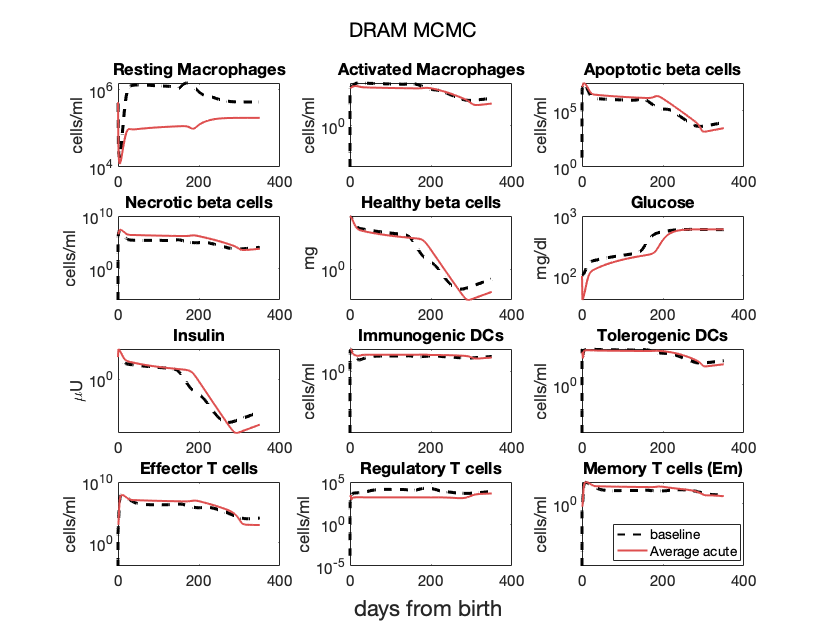
\includegraphics[width=15cm]{MCMC_figs/dram_t1d_final/allState_mouse6.png}
    \caption{State predictions using parameter values fitted using the DRAM parameterization on Mouse 6 data. Predictions are plotted in red and the dashed line indicates the baseline, pre-parameterized evaluation of the particular state. The DRAM algorithm produces biologically feasible results for all 12 states evaluated.}
    \label{fig:dram_biocheck1}
\end{figure}

\begin{figure}[H] 
    \centering
    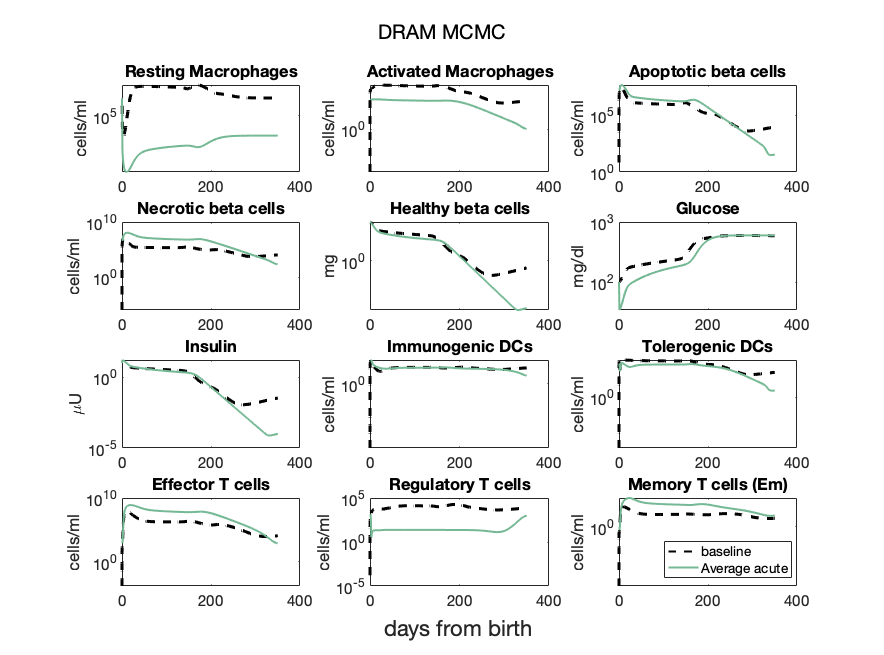
\includegraphics[width=15cm]{MCMC_figs/dram_t1d_final/allState_avg.png}
    \caption{State predictions using parameter values fitted using the DRAM parameterization on average acute data. Predictions are plotted in green and the dashed line indicates the baseline, pre-parameterized evaluation of the particular state. The DRAM algorithm produces biologically feasible results for all 12 states. However, the prediction for Resting Macrophages is significantly different from the baseline.}
    \label{fig:dram_biocheck2}
\end{figure}
\begin{figure}[H] 
    \centering
    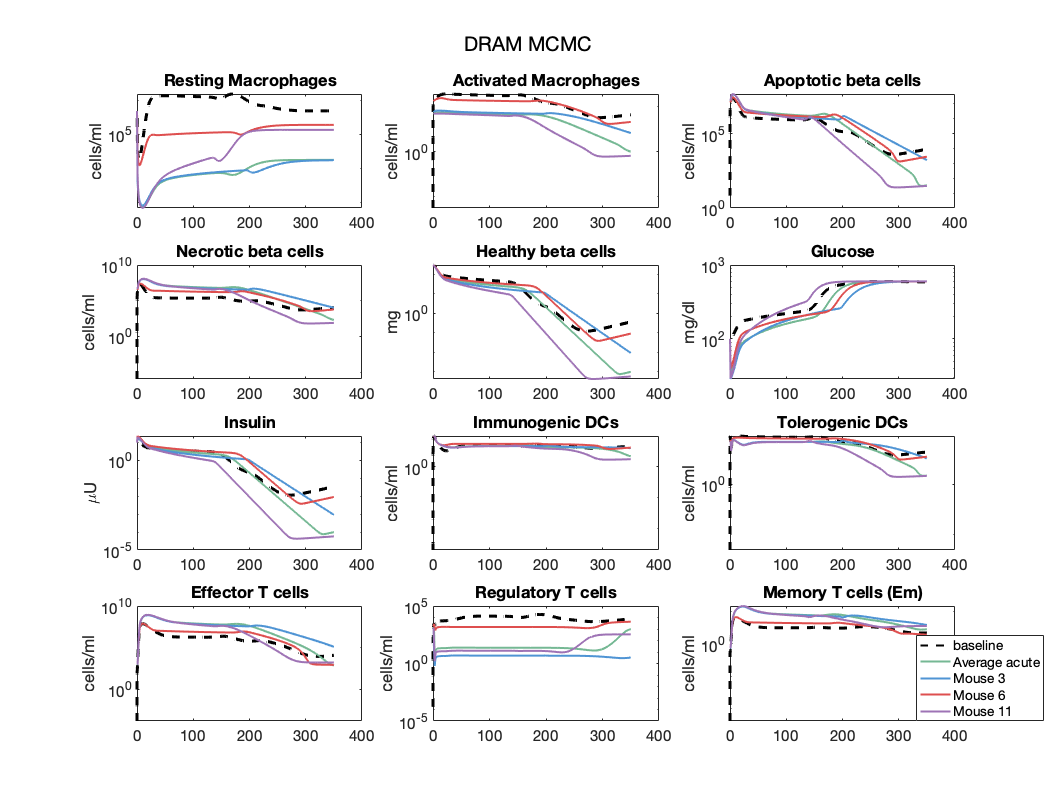
\includegraphics[width=15cm]{MCMC_figs/dram_t1d_final/allState_comp_3_6_11_avg.png}
    \caption{State predictions using parameter values fitted using the DRAM parameterizations on Mice 3, 6, 11 and average acute data. Predictions are plotted in solid colors and the dashed line indicates the baseline, pre-parameterized evaluation of the particular state. The DRAM algorithm produces biologically feasible results for all 12 states evaluated in each parameterization. The Resting Macrophages and Regulatory T cells predictions show the largest difference from the baseline values.}
    \label{fig:dram_biocheck3}
\end{figure}


\subsection{Notes on the Geweke Diagnostic} \label{appendix:gewekediagnostic}
The Geweke diagnostic is a statistical test to determine if a sampling chain has converged (reached a steady state) \cite{geweke1}. In practice the diagnostic is a two-sample Z-test that compares the means of the first 10$\%$ and last 50$\%$ of the chain (see a basic tutorial on Z-tests \textit{\href{https://ncss-wpengine.netdna-ssl.com/wp-content/themes/ncss/pdf/Procedures/PASS/Two-Sample_Z-Tests_Assuming_Equal_Variance.pdf}{here}}). These percentages may change, but 10\% and 50\% are most commonly used and are the default in the \texttt{mcmcstat} library function \texttt{geweke}. If these means are the same or very similar, we say that the chain has converged within the first 10$\%$ of samples \cite{convergediganosticRoy2020}. 
\par The Geweke diagnostic is calculated as follows:
\begin{tcolorbox}
\begin{enumerate}
    \item Let \textit{C} be the sampling chain post-MCMC estimation (all parameter values have been collected) and let $n_C$ be the number of samples in \textit{C}
    \item Let $m_{n_A}$ and $m_{n_B}$ be the means of the first 10\% and last 50\% of \textit{C}
    \item Let $s_A$ and $s_B$ be the spectral estimates$^*$ for the variance of the first 10\% and last 50\% of \textit{C}
    \item Then the Geweke diagnostic for \textit{C} is
    \begin{equation}
        Z_C^{**} = \frac{m_{n_A} - m_{n_B}}{\sqrt{\frac{s_A}{(0.1)(n_C)} + \frac{s_B}{n_C - [(0.5)(n_C)+1]+1}}}
    \end{equation}
\end{enumerate}


* Power spectral density estimates describe how the power of a time series (in this case each sample of \textit{C}) is distributed with frequency. For more information see \cite{Heinzel2002SpectrumAS}. \\
** In all our MCMC parameter estimations, we are estimating multiple parameters and thus \textit{C} is often a $p$-by-$n_C$ matrix where $p$ is the number of parameters. The calculation of $Z_C$ can easily be used to calculate individual Geweke values for each parameter: $m_{n_A}$, $m_{n_B}$, $s_A$, and $s_B$ are now matrices and operations are performed component-wise.

\textit{Based on definitions from \cite{convergediganosticRoy2020} and the \texttt{mcmcstat} library function \texttt{geweke} \cite{mcmcstatlib}.}
\end{tcolorbox}
\vspace{3mm}
\par Now that we can compute the Geweke diagnostic, we have to interpret it's meaning in order to determine convergence of a chain. As the diagnostic is a simple statistical test, we use conventional methods of analysis. We will use hypothesis testing and p-values to determine significance of Geweke values. Find a brief introduction to hypothesis testing \textit{\href{https://www.statisticshowto.com/probability-and-statistics/hypothesis-testing/}{here}}.\\

\begin{tcolorbox}[colback=red!5,colframe=red!75!black,title=\textbf{Hypothesis Testing}]
Briefly, hypothesis testing is the fundamental idea behind most statistical analyses. We are testing to see if a certain statement is true:
\begin{center}
    \texttt{The chain has converged}
\end{center}
which is our \textit{null hypothesis}. Our \textit{alternative hypothesis} is
\begin{center}
    \texttt{The chain has \textit{not} converged}
\end{center}
We run an experiment to collect some data
\begin{center}
    \texttt{The DRAM MCMC parameter estimation method}
\end{center}
We perform a statistical test
\begin{center}
    \texttt{A two-sample Z-test (Geweke diagnostic)}
\end{center}
We compute a p-value for this statistical test and determine a significance threshold
\begin{center}
    \texttt{Often 0.05}
\end{center}
\end{tcolorbox}
\vspace{3mm}
\par We now briefly review the definition and role of a p-value for the Geweke diagnostic
\begin{tcolorbox}[colback=blue!10,colframe=blue!25!black,title=\textbf{Calculating p-values}]
\begin{enumerate}
    \item Let's say we want to be 95\% sure that we do not state non-convergence when the chain actually has converged (this is also called a false negative and a Type 1 error), then we choose a significance level of $\alpha = 0.05$. 
    \item A \textit{p-value} is the smallest $\alpha$ for which the observed data indicates that we \textit{reject} our null hypothesis. That is, if our p-value is greater than this $\alpha$ threshold, we \textit{fail to reject} the null hypothesis and there is evidence (from the data) to support the alternative hypothesis.
    \item The actual calculation of p-values depends on the statistical test being performed. They are also often calculated by computer programs.
\end{enumerate}
\textit{A brief explanation of p-values is found \textit{\href{https://www.statsdirect.com/help/basics/p_values.htm}{here}}}
\end{tcolorbox}

\vspace{3mm}
\par Now we have the knowledge to calculate Geweke diagnostic values, their p-values, and to interpret the p-values. Let's do an example.
\begin{tcolorbox}[colback=green!10,colframe=green!25!black,title=\textbf{Calculating and Interpreting Geweke Diagnostic values}]
\begin{enumerate}
    \item Our null hypotheses are that the chain has converged for the parameters $\delta_B$ and $\mu_R$.
    \item We choose an $\alpha$ of 0.05 (p-value significance threshold).
    \item We begin with a parameter estimation of the T1D model using DRAM MCMC with the averaged data set. 
    \item We calculate the Geweke diagnostic and p-values for each parameter
    \begin{table}[H]
        \centering
            \begin{tabular}{c|c c}
               & \textbf{Geweke} & \textbf{p-value}\\
            \hline
            $\delta_B$ & 0.0248 & 0.98022 \\
            $\mu_R$ & -2.1923 & 0.028361
            \end{tabular}
    \end{table}
    \item We interpret these p-values. For $\delta_B$ we \textit{fail to reject} our null hypothesis because the p-value $< 0.05$. For $\mu_R$ we \textit{reject} our null hypothesis because the p-value $< 0.05$ and there is evidence to support the alternative hypothesis.
\end{enumerate}

\end{tcolorbox}

\subsection{Notes on running DRAM with \texttt{mcmcstat}} \label{appendix:runningDRAM}
\subsubsection{Efficiency}  We have been able to run both the Metropolis and DRAM algorithms on our local machines (laptops). However, in general, the DRAM algorithm takes more processing time as it runs through extra steps. In addition, we note that the Lotka-Volterra is very simple, only 2 differential equations, with 4 parameters, however, in models with a greater number of equations and parameters, such as the T1D model, the DRAM process can take upwards of an hour to run on a normal laptop. If you are concerned about computing power, we would recommend running these algorithms on a computer cluster.
\subsubsection{User options}
The function \texttt{mcmcrun} that implements the DRAM algorithm, allows several options for specifying a prior function. If left unspecified, a uniform prior is assumed, with its bounds located at the upper and lower bounds of the parameter means and standard deviations specified by the user.
\par There also exist several options for specifying estimates for the prior's variance and mean (to be used in the default log-uniform prior). We have not fully explored these, opting instead to write our own prior functions.

\section{PSO} \label{PSO_appendix}
\subsection{Biological Feasibility}
\subsection{Notes on Convergence}




\section{UKF} \label{UKF_appendix}
\subsection{Notes on Implementing the UKF}
\subsubsection{Biological Feasibility}
Recall that in Section \ref{biocheck_dram}, we evaluated the performance of the DRAM parameterization of the Type 1 diabetes model using Mouse 6 data for 4 of the 12 ODE states. Here we present the full 12 state predictions from parameterizations on Mouse 6 for both the Dual and Joint UKF.\\

First, we present the Dual in Figure \ref{fig:Dual_ALLSTATES_Wave}. Here, the model is run with the apoptotic wave turned on.

\begin{figure}[H] 
    \centering
    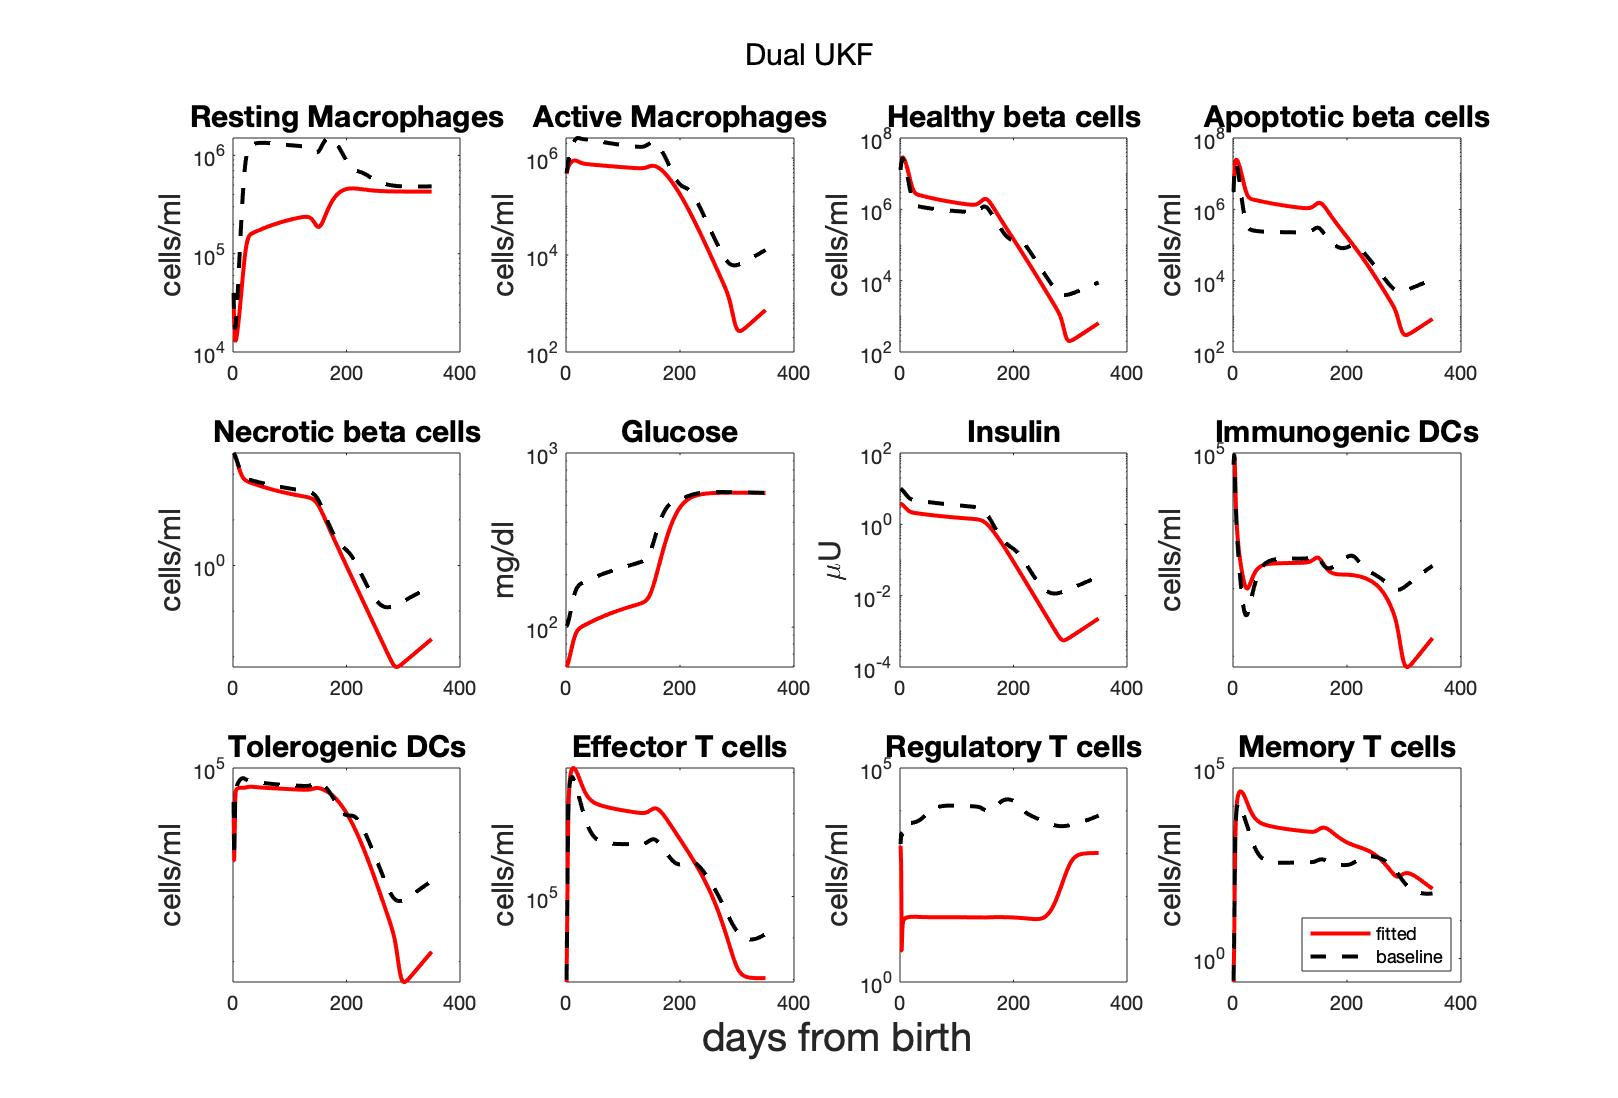
\includegraphics[width=15cm]{Kalman_Filter_Images/States_With_Wave_ALL_WithBaseline.jpg}
    \caption{State predictions using parameter values fitted using the Dual UKF parameterization on Mouse 6 data. Predictions are plotted in red and the dashed line indicates the baseline, pre-parameterized evaluation of the particular state. Results appear feasible for all states, however the Regulatory T Cell behavior deviates significantly from the baseline.}
    \label{fig:Dual_ALLSTATES_Wave}
\end{figure}

Analogously, Figure \ref{fig:Dual_ALLSTATES_NoWave} displays all 12 states when the model is run with no apoptotic wave.

\begin{figure}[H] 
    \centering
    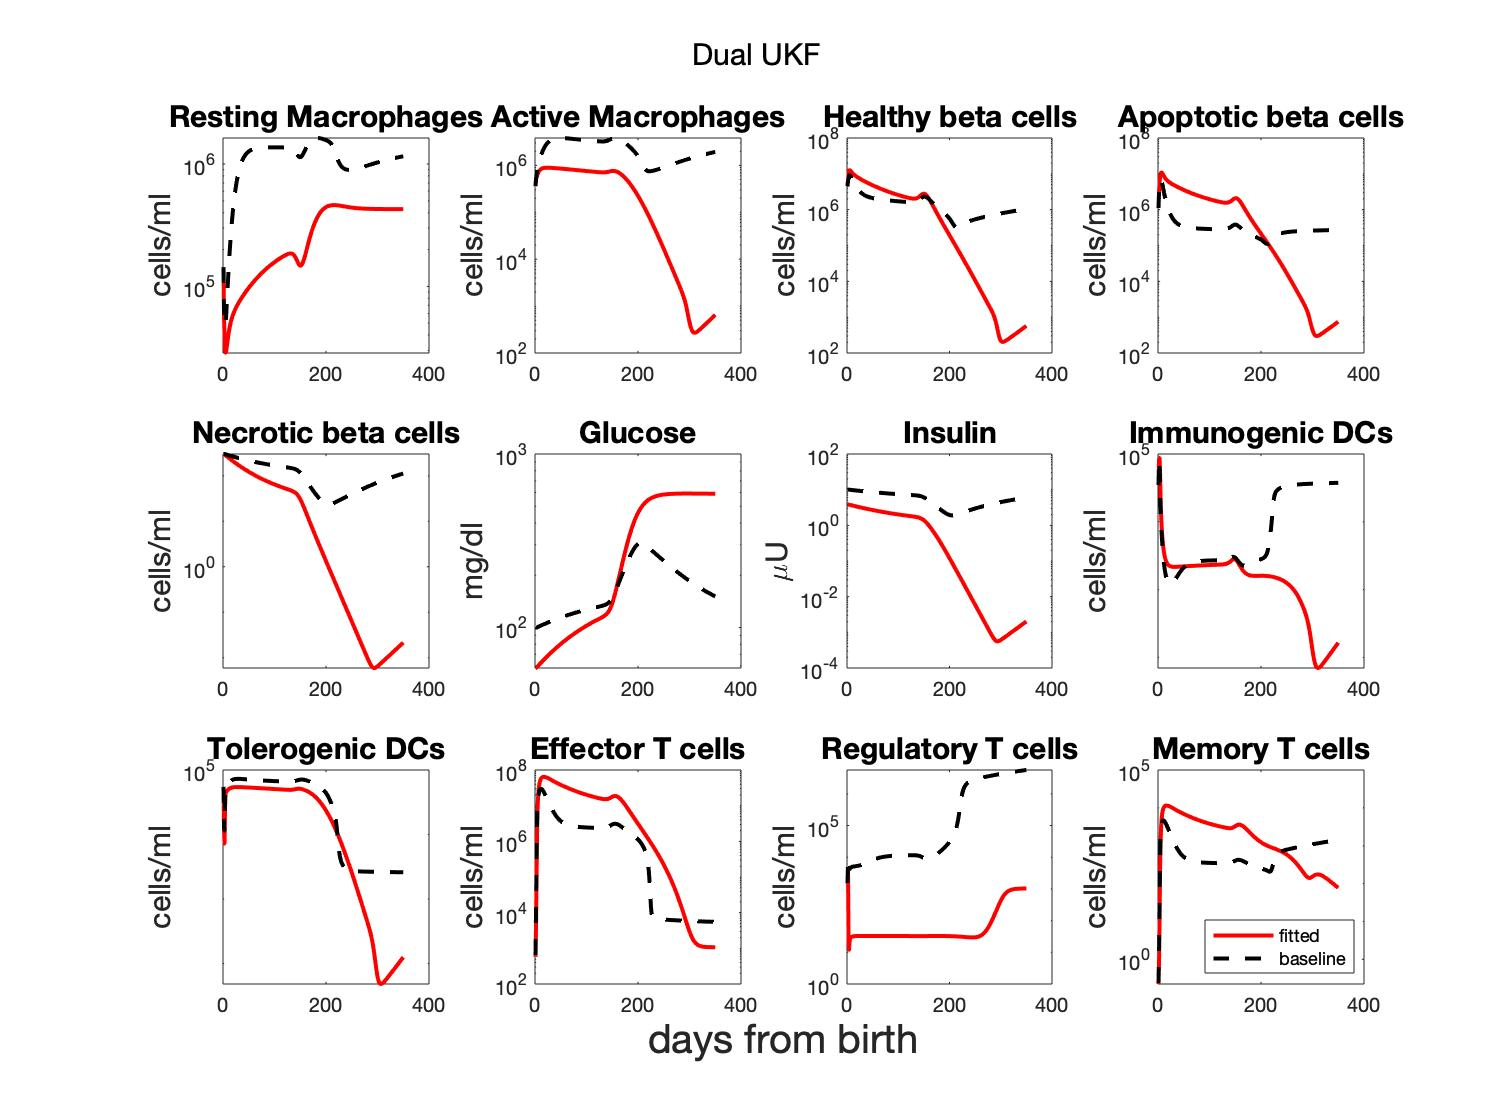
\includegraphics[width=15cm]{Kalman_Filter_Images/States_NOWAVE_ALL_withBaseline.jpg}
    \caption{State predictions using parameter values fitted using the Dual UKF parameterization on Mouse 6 data when no wave is present. Predictions are plotted in red and the dashed line indicates the baseline, pre-parameterized evaluation of the particular state. Unfortunately, as seen in the Glucose panel, the mouse still reaches an unhealthy steady state in our simulations.}
    \label{fig:Dual_ALLSTATES_NoWave}
\end{figure}


We now present similar figures for the Joint. First, we have the states when the wave is present:

\begin{figure}[H] 
    \centering
    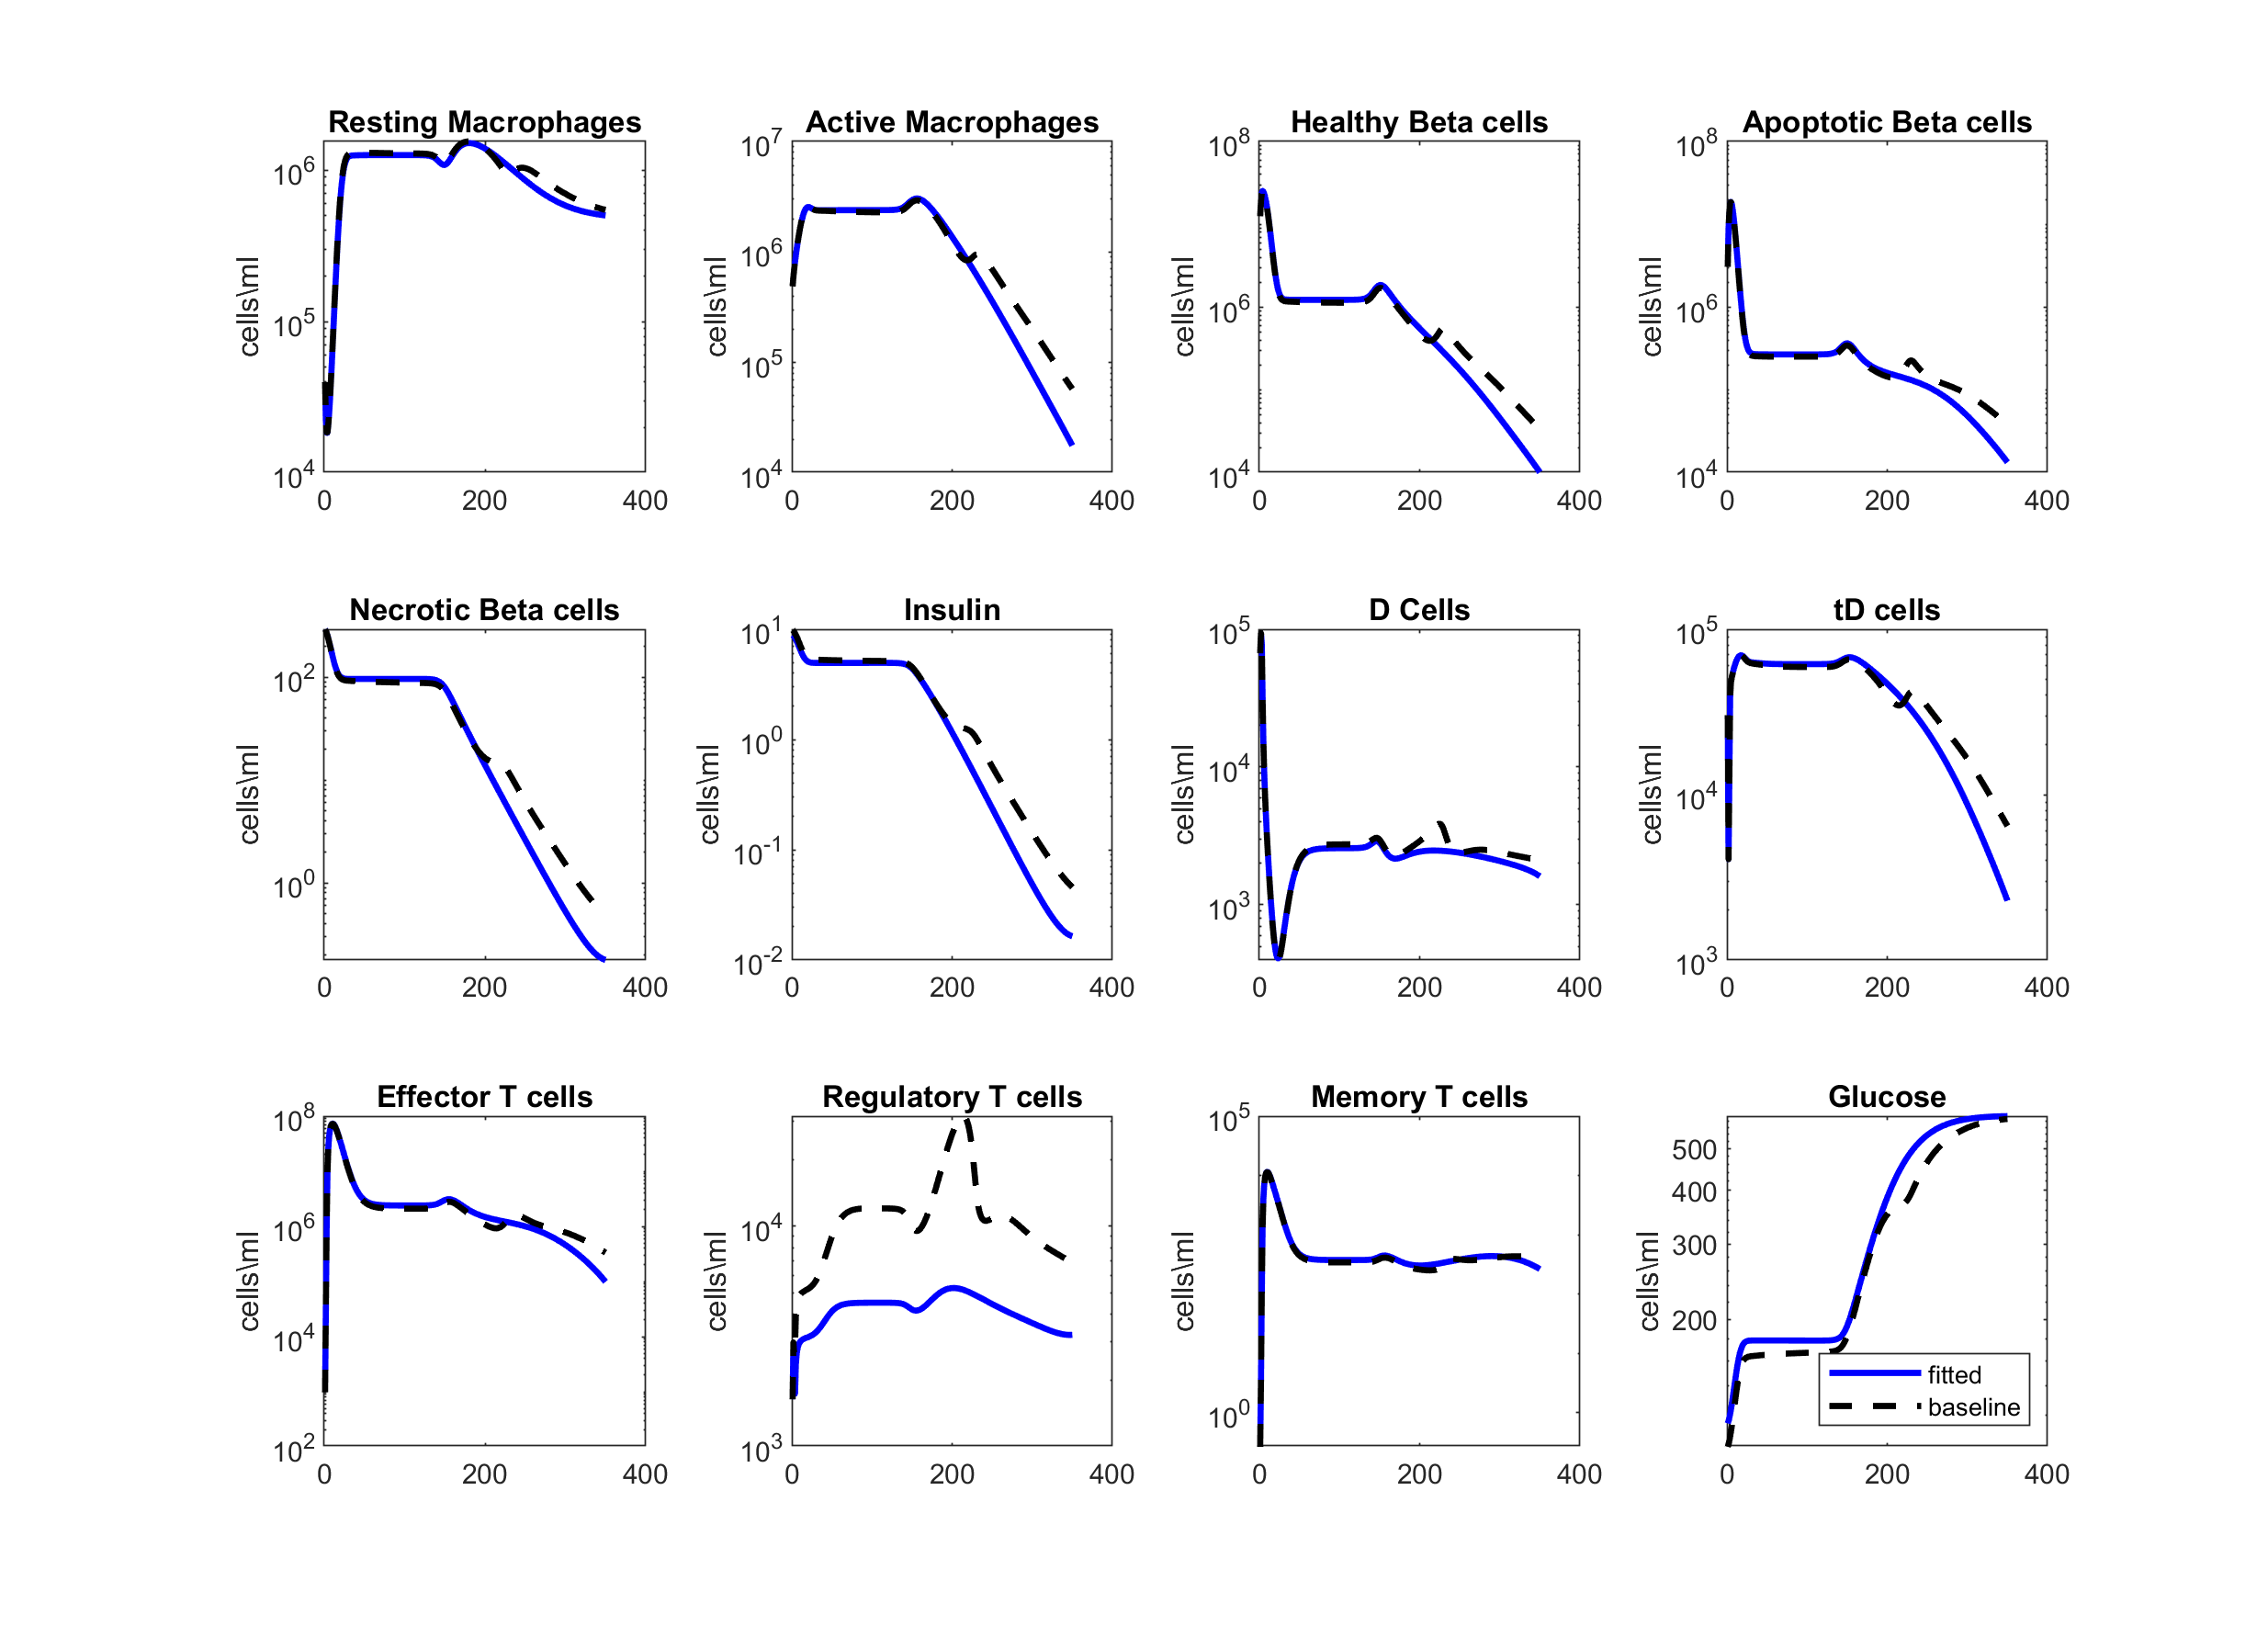
\includegraphics[width=15cm]{Kalman_Filter_Images/Joint_mouse6_allstates.png}
    \caption{State predictions using parameter values fitted using the Joint UKF parameterization on Mouse 6 data. Predictions are plotted in red and the dashed line indicates the baseline, pre-parameterized evaluation of the particular state. The Joint UKF algorithm produces biologically feasible results for all 12 states evaluated, although Regulatory T Cells are notably about an order of magnitude off.}
    \label{fig:ukf_biocheck1}
\end{figure}
Next, we have the states when the wave is not run:
\begin{figure}[H] 
    \centering
    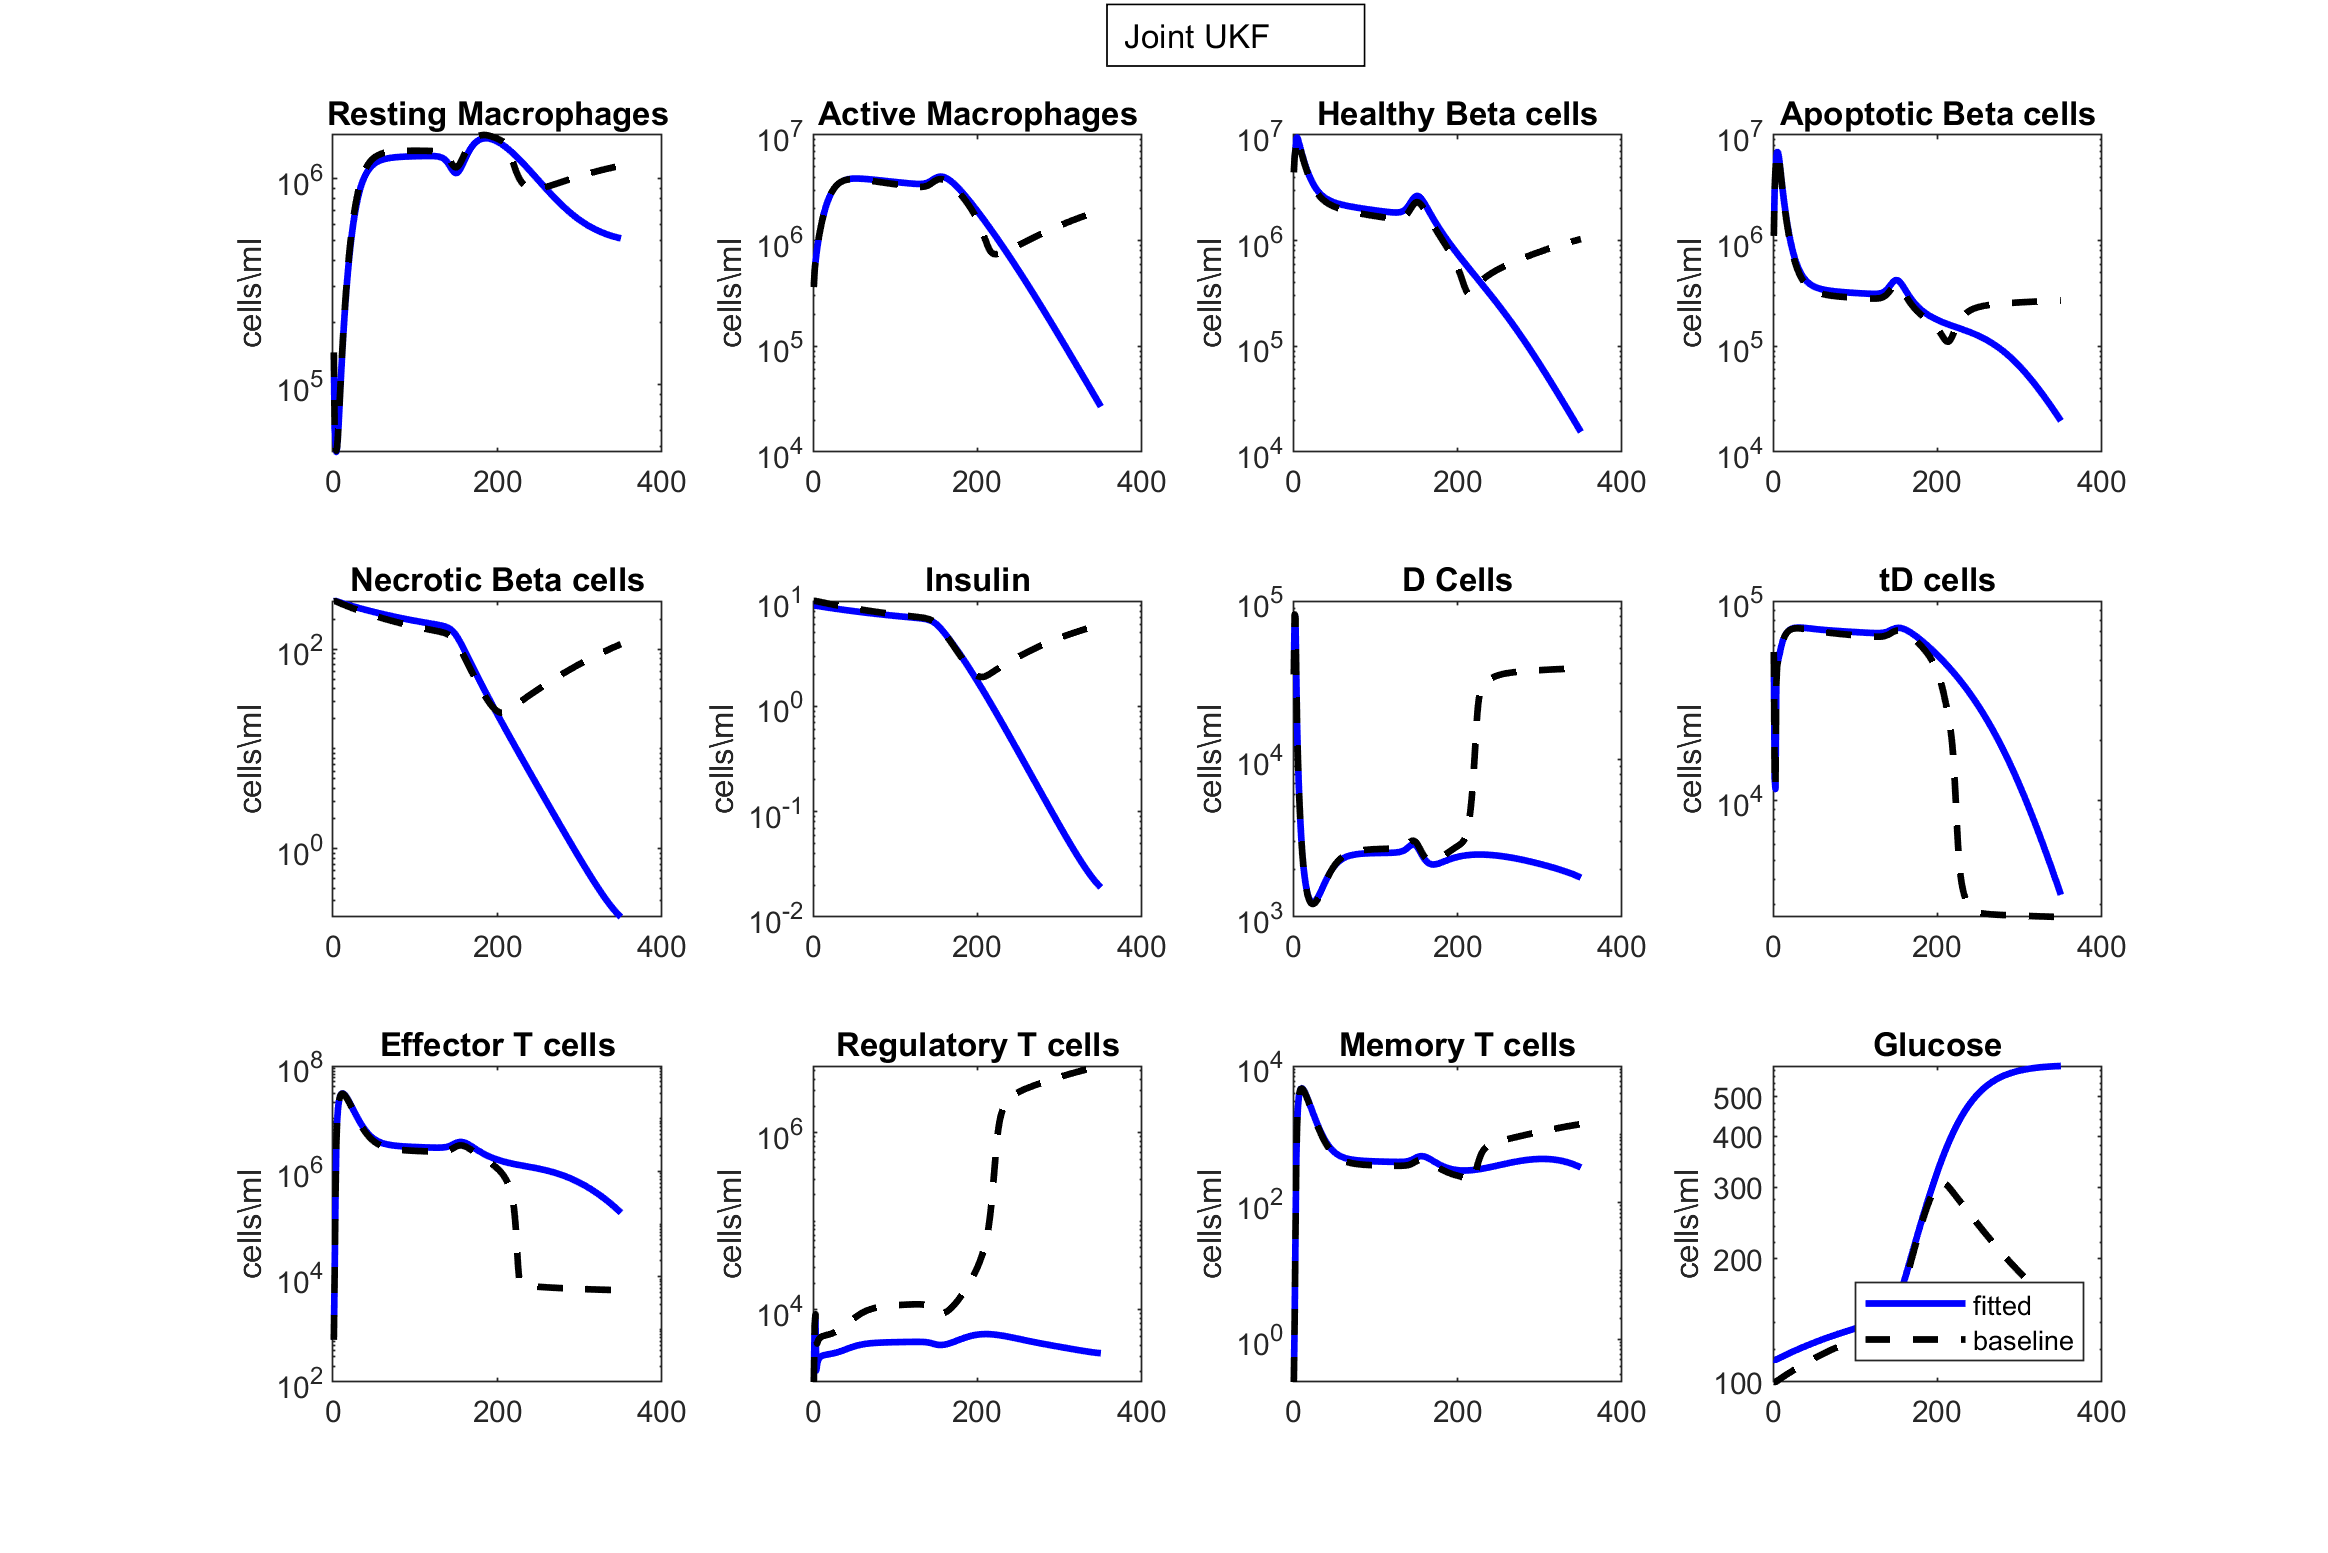
\includegraphics[width=15cm]{Kalman_Filter_Images/Joint_mouse6_allstates_nowave.png}
    \caption{State predictions using parameter values fitted using the DRAM parameterization on Mouse 6 data. Predictions are plotted in red and the dashed line indicates the baseline, pre-parameterized evaluation of the particular state. The Joint UKF algorithm produces biologically feasible up to a point, but at a specific time point, likely when the apoptotic wave would occur, most of the baseline predictions for the states experience a sharp shift that the fitted results cannot replicate.}
    \label{fig:ukf_biocheck2}
\end{figure}

\subsubsection{Parameter Bounds}
Oftentimes, it can be useful to create a step in the UKF algorithm that checks that the parameters are within some biologically feasible bounds, and if they are not, keep the previous estimate. This can be especially important for making sure parameters are positive. Not only is is usually biologically infeasible for a parameter to be negative, having negative parameter values can interfere with the running of the filter. 




\end{appendices}